\documentclass[11pt]{article}
% Useful emacs macro for inserting normal quotes when
% Ctrl-c Ctrl-d is pressed.
%
% (fset 'insert_quote
%   "\C-q\"")
% (global-set-key "\C-c\C-d" 'insert_quote)

%include polycode.fmt
\usepackage{palatino}
\usepackage[scaled=0.92]{helvet}
\usepackage{graphicx}
\usepackage{fullpage}
\usepackage{url}
\usepackage{fancyvrb}
\usepackage{qtree}
\renewcommand\ttdefault{cmtt}

\newcommand\FIG{
\includegraphics[width=2in, height=1.5in]{sample}}
\author{Justin Bailey \\ \url{justinb@@cs.pdx.edu} \\ CS506 -- Spring 2009}
\title{Caffeine -- The Habit-Forming Compiler}
\date{}

\begin{document}
\fvset{fontfamily=cmtt}
%if False
\CustomVerbatimEnvironment{code}{Verbatim}{}
%endif
\VerbatimFootnotes
\DefineShortVerb{\#}

\maketitle

\section{Introduction}

Habit is a pure, functional language that looks a lot like
Haskell. Caffeine, described in this report, compiles a subset of the
Habit language into executable programs for the x86 platform. Though
the semantics of Habit have not been formalized, we treat it as a
strict language and compile accordingly. In broad strokes, Caffeine
consumes an AST produced by the front-end parser and transforms it to an
intermediate language (IL) targeting a simple register machine. The
IL is transformed to x86 assembly code, #gcc# is used to link our 
output into a small runtime, and an executable is produced.

The current implementation has no I/O capabilities and no support for
primitive types (e.g., integers). Programs with algebraic data types
performing pure computation are supported, however. Therefore, we'll
use the |foldr| function over lists as a running example. As there is no syntax
support for lists yet, we define them
first:\footnote{Habit's syntax looks a lot like Haskell's. In fact, the
  portion implemented by Caffeine is exactly the same. All the
  examples in this report should be readable by anyone familiar with
  Haskell.}

\begin{code}
  data List a = Cons a (List a) | Nil
\end{code}

\noindent
Pattern-matching allows us to define |foldr|:

\begin{code}
foldr :: (a -> b -> b) -> b -> List a -> b
foldr f b Nil          = b
foldr f b (Cons a as)  = f a (foldr f b as)
\end{code}

\noindent
We also define a data type for natural numbers, using Peano representation:

\begin{code}
  data Nat = S Nat | Z
\end{code}

\noindent
Now we can define operations like |add| on our |Nat| type:

\begin{code}
  add :: Nat -> Nat -> Nat
  add Z b      = b
  add (S a) b  = S (add a b)
\end{code}

\noindent
With these functions in place, we can now define |sum| over a list of
|Nat|s:

\begin{code}
  sum :: List Nat -> Nat
  sum = foldr add Z
\end{code}

In the following section of the report, we detail the representation
of function and data values, how allocation is accomplished and how
function definitions, especially recursive ones, are
translated. Section \ref{sec_code_generation} then details how code is
generated. We start by describing the translation from Habit to the IL
for the register machine, and then show the
translation from that language to x86 assembler. Throughout the
functions defined above are used as our running example.

\section{Compilation Overview}

\subsection{Function Definitions \& Application}
\label{subsec_function}
Caffeine assumes all functions take one argument and return a
value. For example, |foldr| is treated as if it were defined as
follows\footnote{In fact, the front-end performs just this kind of
  transformation.}:

\begin{code}
  foldr = \f -> \b -> \rest -> 
    case rest of
        Nil          -> b
        (Cons a as)  -> f a (foldr f b as)
\end{code}

For example, the expression:

\begin{code}
foldr f Z (Cons Z Nil)
\end{code}

\noindent
has the AST representation shown in figure
\ref{fig_AppExample}. \verb=@= represents function application, with the function
on the left and the argument on the right. Evaluating each node, except the
topmost, results in another function. Only evaluation of the topmost
node actually results in the body of |foldr| executing. 

\begin{figure}[h]

\Tree [.@@
         [.@@
           [.@@
             |foldr|
             |f|
           ]
           |Z|
         ]
         [.@@ 
            [.@@
               |Cons|
               |Z|
            ]
            |Nil|
         ]
      ]
\caption{A graphical representation of the AST for |foldr f Z (Cons Z Nil)|.}
\label{fig_AppExample}
\end{figure}

This same scheme is also used for data constructors. Each constructor
is treated as a function and the same representation is built for
them. In fact, data constructors are functions except their body
contains a primitive operation for creating the data value. 

Every function application generates more-or-less the same code. If a
function takes $n$ arguments, then $n - 1$ intermediate ``functions'' will
be generated. Each function does the same thing:

\begin{enumerate}
  \item Create a closure to pass to the next function.
  \item Copy all values from the current closure to the new.
  \item Copy the argument to the current function into the new closure.
\end{enumerate}

Each intermediate function consumes one argument until only one
remains. The function body then executes in an environment where all
free variables and arguments (except the last one) are stored in the
closure received. 

This represention, while inefficient, allows for a uniform treatment
of application: every function takes one argument and returns some
value. This uniformity defines a ``protocol'' and allows the same code
to be generated for all applications, with no special cases. Clearly,
opportunities for optimization exist here, but have not yet been
exploited. For example:

\begin{itemize}
  \item If all the arguments to a function are present in a given
    application, the intermediate functions could be skipped.
  \item If a value is never used, it should not be propogated through
    each closure. 
\end{itemize}

\subsection{Recursive Functions}

The first step in the process above is free variable analysis on the
function definition. Appropriate code is generated to ensure all free
variables are copied into the closure and located somewhere in the
environment. Recursive functions present a special challenge, for one
of two reasons: the function's recursive call appears to be free or
we must place the function in the environment before it is defined.

Caffeine handles this problem by first analyzing all declarations for
recursion.\footnote{Technically, the front-end implements this by
  representing recursion as edges on a graph between declarations and
  finding the strongly-connected components.} Recursive functions are
assigned a location in the environment first. The body of each is then
compiled. Because the function is in the environment already, recursive
calls are no different than any other function application.

Mutually recursive functions present an additional challenge. Not only
must they be defined before they are compiled, each function will
expect to find the others in their local environment. That means the
compiled code must allocate the closures referring to each function
together and copy those closures into each other. In this situation,
compilation proceeds as above. The allocation of the initial closure
for each function, however, is collected separately. Those allocations
are placed together so that subsequent loads into the closures occur
after the allocation has occurred.

For example, consider this pair of recursive functions:

\begin{code}
  main = 
       let  even Z      = True
            even (S n)  = odd n
            odd Z       = False
            odd (S n)   = even n
       in odd (S (S Z))
\end{code}

When |even| is compiled, |odd| appears free. Similarly, |even| is free
in |odd|. Therefore, the closures for each must appear in the
other. Caffeine follows these steps to allocate and initialize the
closures correctly:

\begin{enumerate}
 \item Allocate closure for |even|, call it #cloEven#.
 \item Allocate closure for |odd|, call it #cloOdd#.
 \item Store the address of #cloOdd# in the first slot of #cloEven#.
 \item Store the address of #cloEven# in the first slot of #cloOdd#.
 \item Evalute |odd| with the argument |S (S Z)|.
\end{enumerate}

The two closures are each allocated with one slot, since they have one
free variable. The address of each closure is then copied into the
other. This ensures that by the time either function is entered, the
location of the other is well-defined.

\subsubsection{Recursive and Circular Data Values}

Recursive data types, such as the |Nat| type used in previous
examples, are much simpler than recursive functions. Given that we
compile Habit with an eager evaluation strategy, all values (even
recursive ones) are present when a given constructor function is
evaluated. There are no ``forward'' references to worry about when
evaluating the body of a constructor.  

Circular data values, where a
value refers to itself, are a different story. Fortunately, they are
impossible to create using Caffeine. Some sort of mutable reference
would need to be implemented before such a
program could be produced.

\subsubsection{Mutually Recursive Values}

Mutually recursive values, under eager evaluation, are not easy to
support. Caffeine does not compile such programs correctly. The
following example will compile but produces strange results:

\begin{code}
  main = 
     let  f        = S g
          g        = S (S f) 
          h (S n)  = (S Z)
          h Z      = Z
     in h g
\end{code}

\subsection{Global Declarations}
\label{subsec_global}
The above examples used locally defined functions. That choice was
made because otherwise each function would not appear free
in the other's environment! Caffeine treats top level, or global,
declarations differently during free variable analysis.\footnote{Global
  declarations are defined as those with ``module'' qualified
  names.} Since those definitions can
be  located at compile time, there is no need to copy them into
the closure of functions that refer to them. Therefore, such
declarations are excluded from free variable analysis. If |odd| and
|even| had been declared at the top level, the compiler would have
only produced the allocation of two nullary closures. This
optimization is described in more detail in section
\ref{subsubsec_compile-time_allocation}.

\subsection{Closure and Data Representation}
\label{subsec_closure}
There are two kinds of values allocated by the compiler: closures and
structured data values. Both are allocated on the heap and have a
uniform representation. Each object begins with a header word,
followed by a variable number of word-sized slots. For constructors,
the number of slots equals the number of arguments to the
constructor. For closures, the number of slots is equal to the number
of arguments to the target function, less one. This closure structure
is due to the way function application is compiled, and is explained in
section \ref{subsec_function}. Graphically, heap
objects have the structure shown in figure \ref{fig_Heap}.

\begin{figure}\centering
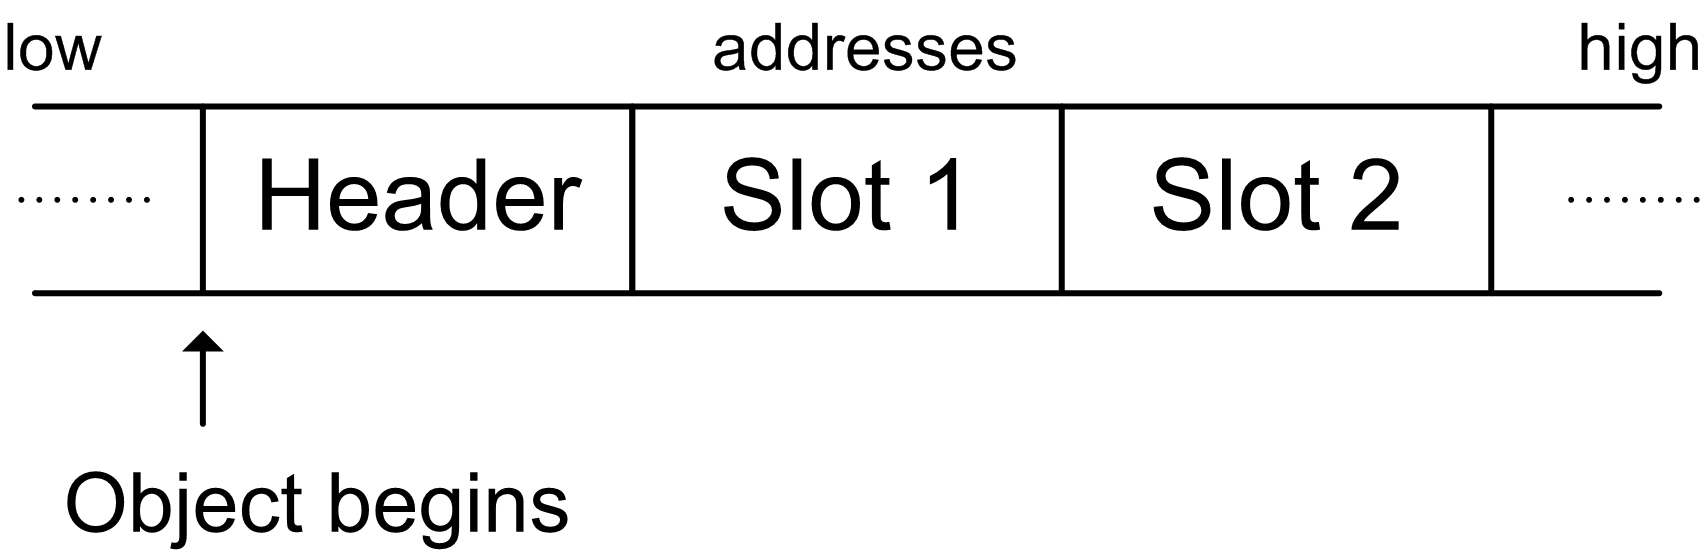
\includegraphics{fig_Heap}
\caption{This figure illustrates the layout of heap objects.}
\label{fig_Heap}
\end{figure}

The value found in the header word of the object is an address. When
the object is a closure, the address is the beginning of the target
function. For a data value, the address holds a tag indicating the
constructor used to create the value.

\begin{figure}\centering
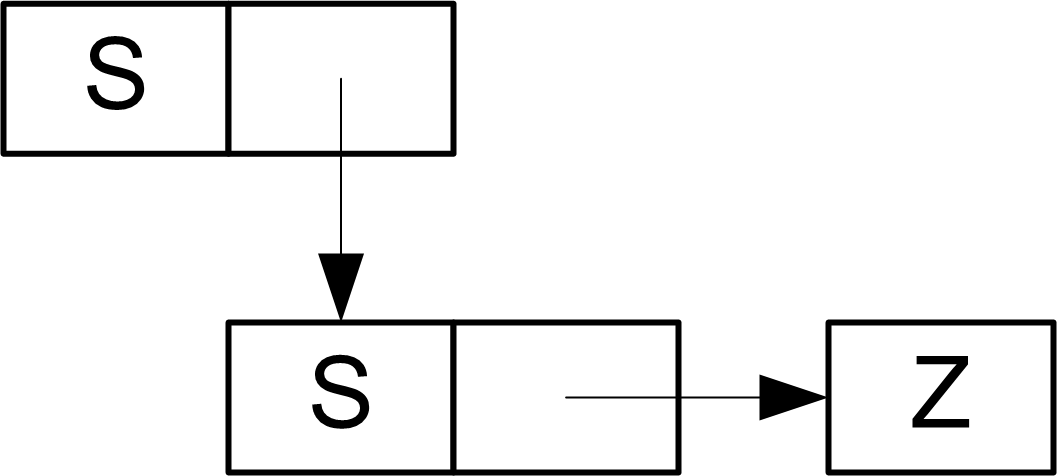
\includegraphics{fig_HeapExample}
\caption{The layout of the value |S (S Z)| in the heap.}
\label{fig_HeapExample}
\end{figure}

Referring to our |Nat| definition above, the value |S (S Z)| would be
represented as in figure \ref{fig_HeapExample}. Each slot in the object holds
an address which points to another allocated object. Each value
ultimately points to some constructor definition.

As said, the address in the header word refers to either a destination
function or a data constructor. Preceeding that address in memory is
an ``info table,'' which holds information describing the function or
constructor. Three pieces of information are found there:

\begin{itemize}
  \item \emph{Size} -- The expected size of the closure or the number of
    arguments for the data constructor.
  \item \emph{Constructor Flag} -- A flag indicating if the definition
    is for a data constructor or not.
  \item \emph{Constructor Name} -- An address referring to a string
    holding the name of the constructor.
\end{itemize}

The last two items are used for debugging or printing results and
the last is only present when the definition is for a data
constructor. It is important to remember that this structure is
created at compile time and becomes part of the program's assembly
code.

The values are laid out in reverse order, with ``size'' preceding the
address, followed by the ``data constructor'' flag, and so on. For
example, figure \ref{fig_SDef} illustrates the |S| constructor from
earlier. ``#regFoldr_S#'' is a label representing an address, at which
the definition of the constructor appears. The prior word, 
#regFoldr_S#$ - 1$, holds the
number of arguments expected by the constructor (1 in this
case). #regFoldr_S#$ - 2$  holds a 1, indicating the this definition is a
constructor. Finally, #regFoldr_S#$ - 3$ holds a pointer to a string with
the constructor's name.

\begin{figure}\centering
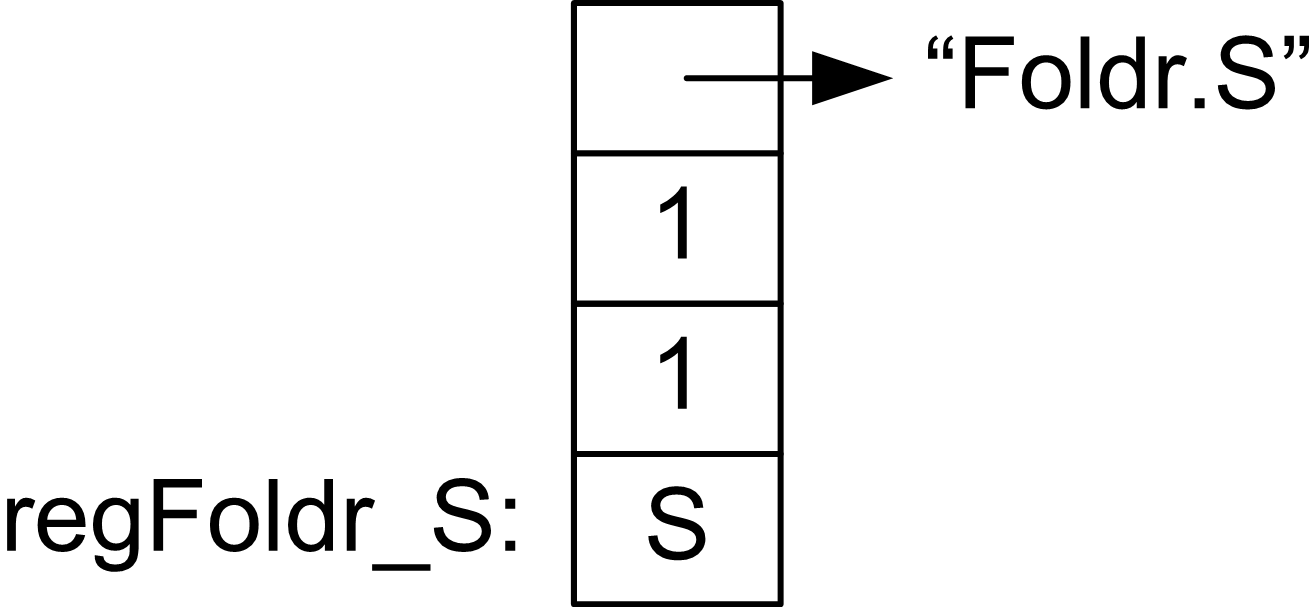
\includegraphics{fig_SDef}
\caption{The info table for the |S| constructor.}
\label{fig_SDef}
\end{figure}

A closure looks much the same. Figure \ref{fig_foldr_Layout} illustrates the
definition of the |foldr| function from above. ``#lab23#'' is again a
label representing the address at which the definition of |foldr|
appears. #lab23#$ - 1$ gives the number of arguments expected in the
closure (2 in this case). #lab23#$ - 2$ holds 0, as this is not a data
constructor. The info table does not extend to #lab23#$ - 3$,
since that only applies to data constructors.

\begin{figure}\centering
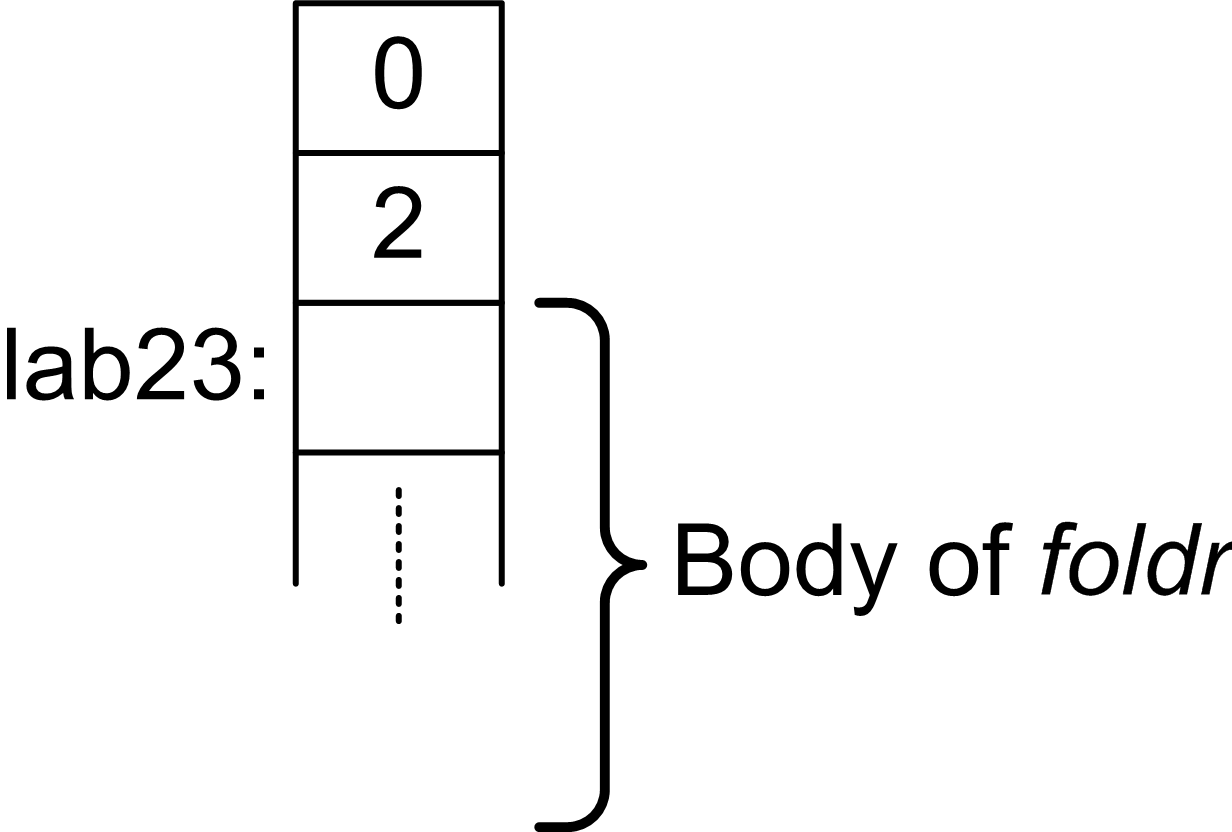
\includegraphics{fig_foldr_Layout}
\caption{The info table for |foldr|.}
\label{fig_foldr_Layout}
\end{figure}

\subsection{Allocation}
\label{subsec_allocation}
The info table's primary role is to assist the runtime in allocating
heap objects. The runtime uses the size field to determine how much
heap space should be allocated for a given data value or closure. 

This scheme allows for an interesting optimization of zero-argument,
or ``nullary,'' objects. Such an object will only have a head,
pointing to the definition of the object. The address of the
definition is known at compile time. Therefore, nullary objects can
actually be allocated at compile time and placed directly in the
assembly output. 

For example, figure \ref{fig_HeapZDef} shows the assembly
representation of the |Z| constructor and its allocated object. |Z| is defined
at label #RZ# and has the same format as any other constructor. Label
#LZ#, however, is an ``allocated'' object which holds a |Z|
value. This value would be created at runtime and stored in the heap
if the constructor took arguments. Since there are no arguments, we
can ``allocate'' at compile time. #LZ# is a label in the assembly
source which holds a |Z| value (by pointing to the |Z| constructor
definition at #RZ#). Whenever a |Z| value is allocated in the Habit
source, #LZ# will be used. No other allocation of |Z| values will ever
occur.

\begin{figure}\centering
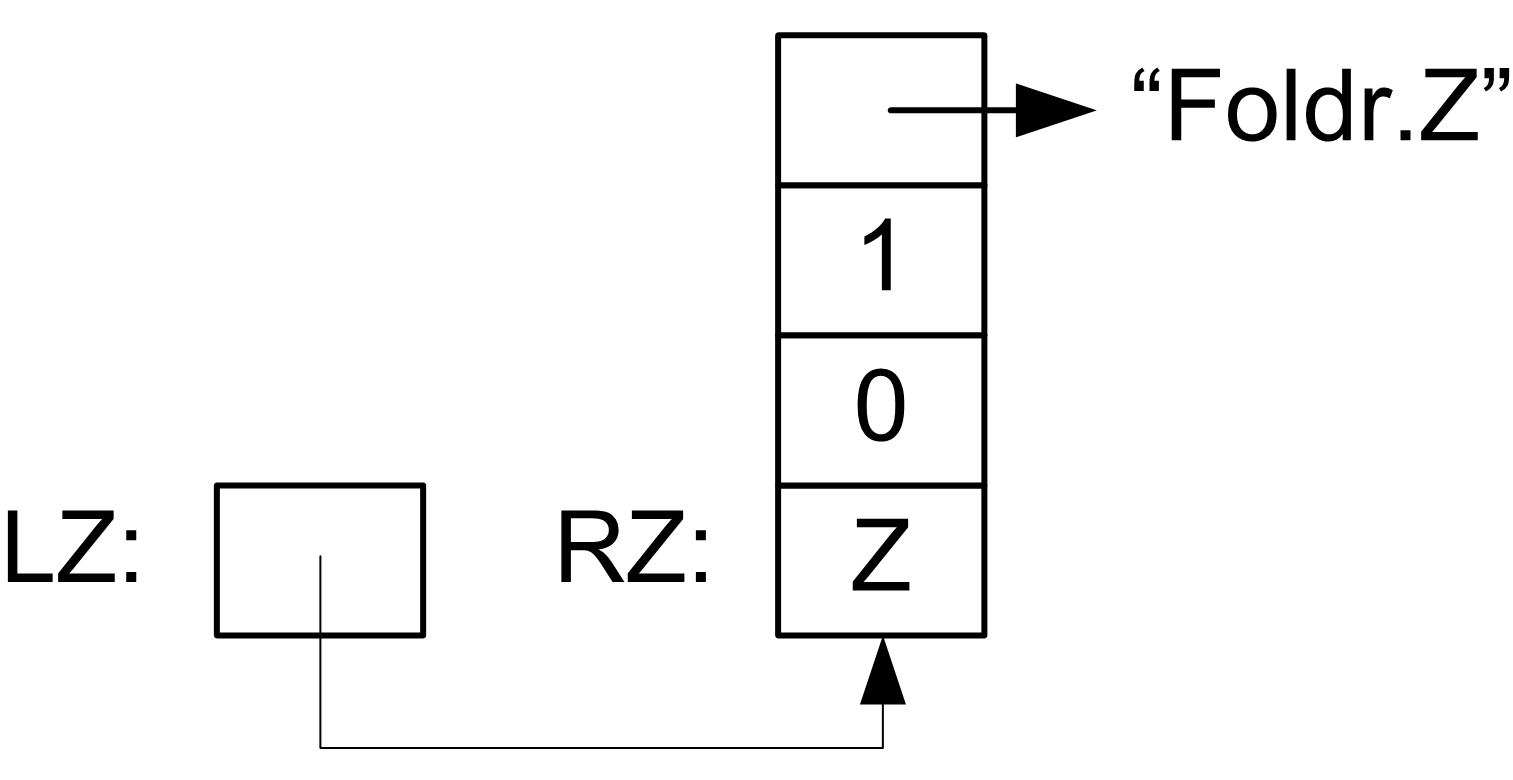
\includegraphics{fig_HeapZDef}
\caption{The definition of the Z constructor and its ``heap'' object are
  shown.}
\label{fig_HeapZDef}
\end{figure}

Nullary values such as |Z| and closures with no arguments never take
heap space, as they are only ``allocated'' once, in the program
text itself. Section \ref{subsubsec_compile-time_allocation} describes
this in more detail.

\section{Code Generation}
\label{sec_code_generation}

Executable code is generated in two steps. The AST produced by the
front-end is compiled to an IL targeting a simple
register machine. The IL program is then compiled
to x86 assembler and linked to the C runtime using #gcc#. The first
step eliminates higher-order functions, generates the ``intermediate''
functions described above, and groups all instructions related to a
particular function definition together. The second step maps virtual
registers to real locations, generates ``compile-time'' closures and
values, and hooks into runtime primitives such as allocation. Each
step is described in detail below.

\subsection{Register Machine \& Intermediate Language}

The IL produced by the first step of
compilation is a program in the ``instruction set'' of the register
machine. It can be described as a first-order, imperative language
with no facility for abstraction. The language does not support
higher-order functions, pattern-matching, algebraic data types, or
other aspects of a ``functional'' language. However, it does support
branching, unconditional jumps, and function calls. 

The machine which ``executes'' the IL has its own model
of computation. It has an infinite supply of registers which can be
used just by naming them. Two special registers always exist,
``#clo#'' and ``#arg#,'' which hold the closure and argument for a
function when it is executed. The machine understands how to allocate
structured data, which can be either closures or data values. Finally,
it is an imperative machine so updates to existing registers will
propogate. In particular, the #clo# and #arg# registers are updated
frequently.

The language and machine were designed together with two goals in
mind. The first was to allow a straightforward mapping to x86 assembly
language, which kept the instruction set simple. The second was to
serve as an intepreter for Habit programs. Programs written in IL can
be executed by the machine. This allowed the compiler to be tested
during development, before executable code could be produced. A suite
of test programs and expected results were developed which ensured
programs continued to execute correctly as the compiler was developed.

\subsubsection{IL Instructions}

The most interesting instructions in the IL are |Enter|, |FailT|,
|AllocC|, and |AllocD|. In brief, |Enter| implements function calls,
|FailT| tests for constructors, |AllocC| creates closures and |AllocD|
creates data values. We'll explore the use of these instructions in
terms of the |foldr|, |sum|, and |Nat| definitions above. 

|AllocC| creates a closure in the register specified. A closure
contains a label, which refers to  the code which will be executed, and
some number of slots holding values:

\begin{code}
AllocC "register" "label" size
\end{code}

\noindent
|Enter| takes three registers as arguments:

\begin{code}
Enter "closure" "argument" "result"
\end{code}

\noindent
The first is the closure which indicates the function to execute and
stores its free variables, the second the argument to the function,
and the last is where the result of the function will be placed. When
an |Enter| is executed, the machine jumps to the instruction referred
to by the label in the closure and begins executing. It returns to the
instruction after the |Enter| when a return (``|Ret|'') is executed.

The |sum| function illustrates these instructions. Recall its
definition:

\begin{code}
sum :: List Nat -> Nat
sum = foldr add Z
\end{code}

\noindent
This compiles to two separate code blocks -- one to enter the function
and one to evaluate the body. To enter the function, we allocate a
closure and call |Enter|:

\begin{code}
  AllocC "globFoldr_sum12" "lab13" 0
  ...
  Enter "globFoldr_sum12" "reg33" "reg34" 
\end{code}

\noindent
#lab13# indicates the body of |sum|, #reg33# holds the list
which is |sum|'s argument (not shown), and #reg34# will hold the
result. Notice that there are no slots allocated for the
closure. Though |foldr|, |add| and |Z| are all free in |sum|, they
are also global declarations and are not included in the closure, as described in
section \ref{subsec_global}.

The body of |sum| compiles to:

\begin{code}
  Enter "globFoldr_foldr16" "globFoldr_add23" "reg55"
  Enter "reg55" "globFoldr_Z0" "reg56"
  Enter "reg56" "arg" "reg57"
  Copy "reg57" "reg58"
  Ret "reg58"
\end{code}

\noindent
The first two |Enter|s prepare a closure for the |foldr| function. The
first passes the |add| function and the second the initial value,
|Z|. The second |Enter| puts its result in #reg56#, which is a closure
that points to the body of |foldr|. The third |Enter| instruction
executes |foldr|, passing the #arg# register as an argument. #arg#
holds with the list given to the |sum| function. The result, which is
the result of the fold, is placed in #reg57#. That value is
copied to #reg58# before being returned. Note that the copy is not
necessary, but due to the lack of optimization in Caffeine.

Another example will help illustrate these instructions. Recall the
definition of |foldr|:

\begin{code}
foldr :: (a -> b -> b) -> b -> List a -> b
foldr = \f -> \b -> \as -> 
          case as of
           Nil           -> b
           (Cons a as')  -> f a (foldr f b as')
\end{code}

\noindent
As with |sum|, a top-level closure is allocated:

\begin{code}
  AllocC "reg_foldr11714" "lab15" 0
  Copy "reg_foldr11714" "globFoldr_foldr16"
\end{code}

\noindent
The initial allocation is a closure for the first lambda in the
definition, while the |Copy| instruction puts that value into the
predefined location for |foldr|. A similar pattern occurs for any top
level function with multiple arguments. In any case,
#globFoldr_foldr16# holds the intial entry point for |foldr|. 

Because |foldr| takes three arguments, two ``intermediate'' functions
are generated. They are not very interesting but we will trace them to
see how they relate to the ``real'' function. In this case, we start
with #lab15# and look for the closure it allocates:

\begin{code}
  Label "lab15"
  AllocC "reg110" "lab111" 1
\end{code}

\noindent
#lab111# contains the next (and last) ``intermediate''. Again, we look
at the closure it allocates:

\begin{code}
  Label "lab111"
  AllocC "reg113" "lab114" 2
\end{code}

\noindent
#lab114# then contains the body of |foldr|:

\begin{code}
  Label "lab114"
  Load ("clo",0) "reg115"
  Load ("clo",1) "reg116"
\end{code}

We start by loading arguments from the closure into registers. The
function to fold is found in the first slot and is loaded into
#reg115#. The initial value is in the second slot and is placed in
#reg116#.\footnote{In the recursive case, this will be the accumulated
  value.} 

The next section illustrates the use of the |FailT| instruction. We
evaluate the case arms in order, so we first check for a |Nil|
constructor in the input list (held in #arg#):

\begin{code}
  FailT "arg" "Foldr.Nil" "lab117"
  Copy "reg116" "reg118"
  ...
  Ret "reg118"
\end{code}

\noindent
If the check succeeds, execution continues and the initial (or
accumulated) value found in #reg116# is returned.\footnote{An
  unnecessary copy happens here.} 

However, if the check fails then execution branches to #lab117#, which
immediately jumps\footnote{Another opportunity for
  optimization.} to #lab118#. We now check #arg# for a |Cons|
constructor:

\begin{code}
  Label "lab118"
  FailT "arg" "Foldr.Cons" "lab121"
\end{code}

\noindent
If the match fails, we go to #lab121#, which should never happen in a
well-typed program. Therefore, |foldr| prepares to make a recursive
call to itself:

\begin{code}
  Load ("arg",0) "reg122"
  Load ("arg",1) "reg123"
  Enter "globFoldr_foldr16" "reg115" "reg124"
  Enter "reg124" "reg116" "reg125"
  Enter "reg125" "reg123" "reg126"
\end{code}

\noindent
First, the head and tail of the list are loaded from #arg#
 into #reg122# and #reg123#, respectively. The three |Enter|
instructions following make up the recursive call to |foldr|. The
first calls an intermediate, which captures the function to fold
(found in #reg115#). The next is another intermediate and captures
#reg116#, which is the accumulated value of the fold so far. Finally,
the last evaluates |foldr| over the tail of the list, found in
#reg123#. 

The head of the list, in #reg122#, and the result value, in #reg126#, 
are then passed to the folded function, in #reg115#:

\begin{code}
  Enter "reg115" "reg122" "reg127"
  Enter "reg127" "reg126" "reg128"
  Copy "reg128" "reg118"
  ...
  Ret "reg118"
\end{code}

\noindent
Two |Enter| instructions occur as one ``intermediate'' function has
been generated for the function to fold. An unnecessary copy occurs
and the result is finally returned.

To illustrate |AllocD|, consider the |ones| function:

\begin{code}
ones _ = (S Z)
\end{code}

\noindent
which just replaces its argument with |(S Z)|. |ones|' body is not
very interesting, as it merely executes the |S| constructor, and is
not shown. 

Recall that constructors with arguments are implemented as
functions. |S|, then, is allocated an initial closure:

\begin{code}
  AllocC "globFoldr_S1" "lab2" 0
\end{code}

\noindent
which has no slots, as no ``free'' variables can appear in a
constructor. Since |S| only takes one argument, #lab2# holds the
implementation of |S|. If it took more arguments, $n - 1$ intermediate
functions would be generated, just like a normal function. In any
case, #lab2# has these instructions:

\begin{code}
  Label "lab2"
  AllocD "regFoldr_S126" "Foldr.S" 1
  Store "arg" ("regFoldr_S126",0)
  Ret "regFoldr_S126"
\end{code}

|AllocD| creates the runtime value with one slot and the tag
|Foldr.S|. The |Store| instruction loads the argument for the |S|
constructor into the slot. The value is then returned.

\subsubsection{Match Compilation}

A distinctive feature of the Habit AST is the |Match| data
type. Conditions, guards, case analysis and pattern-matching are
represented by |Match| values. Even function bodies are represented as
``pure'' matches. In short, the |Match| type is at the heart of the
AST. 

There are five |Match| constructors:

\begin{description}
 \item |MPat| -- Defines a pattern-matching expression which
   can succeed or fail. |MPat|s' can also introduce new bindings and
   are used to define arguments in function definitions. 
 \item |MGrd| -- This match expression has a conditional which
   must be satisfied. If the conditional fails, the match fails. 
 \item |MAlt| -- Takes two matches. If the first one fails to
   match, the second one is tried.
 \item |MFail| -- The match that always fails. Used to
   terminate |MAlt| cases.
 \item |MExp| -- A ``match'' that always succeeds and
   evaluates to its associated expression.
\end{description}

Matches operate primarily through alternatives with guard and pattern expressions. For
example, consider:

\begin{code}
  case expr of
      True -> expr
      False -> expr
\end{code}

Each arm of the case is an |MAlt| value and each pattern an
|MPat|. The body of each alternative is just an expression,
represented by the |MExp| value. The condition itself is evaluated and
bound to a fresh variable.

Ultimately, a match can only fail when a pattern match fails. If this
occurs during evaluation of a |MAlt| branch, execution moves to the
next branch. If no branches remain, execution halts altogether. This
construct is implemented with the |FailT| instruction. 

|FailT| compares the value given with a
specific constructor. If they match, execution continues with the
next instruction. For example, consider this program:

\begin{code}
data V = A | B | C

what A = ...
what B = ...
\end{code}

\noindent
|what| will contain these two |FailT| instructions, which test for
each constructor given:

\begin{code}
  FailT "arg" "Triple.A" "lab9"
  ...
  Label "lab9"
  FailT "arg" "Triple.B" "lab16"
  ...
  Label "lab16"
  Error "Match failure!"
\end{code}

\noindent
Notice also the final label, which will halt the program if no match
is found. This can occur anytime a non-exhaustive pattern match is given.

\subsubsection{Compiling MPats}

|MPat| values can introduce new bindings by ``matching'' against a
variable. The match always succeeds and binds the value to the
name. All function definitions are represented this way. For example,
|map| has this definition in the source text:

\begin{code}
  map f xs = ...
\end{code}

\noindent
but in the AST it appears as a structure of |MPat|s:

\begin{code}
  map = MPat "f" (MPat "xs" (...))
\end{code}

This presents some interesting challenges. When compiling a match all
the arguments must be determined and assigned a location in the
environment. Pattern-matched arguments may have no explicit name but
still must be located. Finally, because each |MPat| can only capture
one argument at a time, functions with many arguments have deeply
nested |MPat| structures. All of this makes determining the environment
in which to compile the match very complicated. 

Our strategy\footnote{Implemented by #compileMAbs# in
  #Compiler\Register\Compiler.hs#.} begins by determining the number of
possible bindings that the match can make. A list of locations for
arguments is then generated. This task is quite simple because
arguments can only appear in the current closure or the argument
register -- a benefit of our ``protocol.'' The free variables in the body are determined and code is
generated to copy free variables and arguments between closures as
needed. When the function body is finally compiled, each |MPat|
encountered will bind its variable to the next location in the list
given. This ensures that each binding will be found in the environment
when needed and that it can be located at run-time.

\subsubsection{Input (AST) / Output (Groups)}
\label{subsec_input_output}
The first step of compilation takes a parsed Habit module as input and
returns a list of |Group|s. A module is defined by the front-end and
constitutes all the declarations found in the source file. A
|Group| is defined by the IL compiler and is a list of labeled code
blocks, where each block is a list of IL instructions.

These blocks are not ``basic blocks,'' in that they can have branches,
jumps and function calls. However, the defining characteristic of a
|Group| is that no jump or branch will have a destination outside the
group. The only way for control to leave a group is through an |Enter|,
|Ret| or |Error| instruction. Additionally, a |Group| only has one entry
point. This is not specifically enforced by the data type, but only
one block in the group will ever be the target of an |Enter|
instruction. In essence, a |Group| holds all blocks that make up a
given function's body. 

This data structure serves two purposes. First, all possible registers
used by a function can be easily determined. This allows the mapping
of virtual registers to real locations to be determined at compile
time. Second, the ``entry point'' block can be treated differently
during compilation. A standard ``prologue'' can be inserted before the
block is translated to assembly, and the x86 compiler can ensure that
all other blocks in the group appear after the entry point.

One group generated by the compiler is special -- the #TOP# group. All
top level values , such as nullary closures and data constructors,
will appear in the #TOP# block.  If a module has a |main| function
defined, code will also be generated to return the value of |main| as the
result of the program.

There are many possible optimizations that could be applied to groups
before they they are compiled to assembly. For example:

\begin{itemize}
  \item Eliminate useless jumps.
  \item Analyze blocks for dead-code elimination.
  \item Remove unnecessary copies.
\end{itemize}

\subsection{x86 Assembly}

Caffeine generates x86 assembly code, suitable for compilation by
#gcc#, from the IL instructions produced in the first step. Each
|Group| produced is processed in order, converting each instruction in
each block to assembly. The assembly produced is divided into two
sections, #data# and #text#. The #data# section holds
compile-time allocated closures, nullary data constructors, global
labels, and data definitions. The #text# sections holds the
program's executable code.

\subsubsection{Functions, Data, and Info Tables}

As described in section \ref{subsec_closure}, info tables are used to
describe function entry points and data constructors. For a function,
the info table details how many arguments will be in the closure. The
assembly generated for the function |foldr f b as = ...| looks
like:\footnote{Note that all assembly code shown uses ``AT\&T''
  syntax, which is what the GNU assembler used by #gcc# understands.}

\begin{verbatim}
    .long 0x0
    .long 0x2
lab114:
\end{verbatim}

\noindent
#lab114# is the label at the start of the body of the |foldr|
function. The prior value, #0x2#, indicates that two arguments are
expected in the closure. The next value, #0x0#, indicates to the
runtime that this is a closure value and not a data constructor.

In contrast, the definition of the |S| constructor has this assembler
representation: 

\begin{verbatim}
L3:
    .asciz "Foldr.S"
    .long L3
    .long 0x1
    .long 0x1
Foldr_S: .long 0x278
\end{verbatim}

#Foldr_S# holds the tag representing the constructor, which is
#0x278#\footnote{Tags are calculated by summing the integer value of
each character. Improvements in this area are obvious.} in this case.
The prior value, #0x1#, indicates that |S| takes one argument. The
next tells the runtime this definition is a data
constructor. Finally, the last holds the address of the text
representation of the constructor (#L3# here). #L3# is defined
immediately preceding and is the string ``#Foldr.S#''.

\subsubsection{Compile-Time Allocation}
\label{subsubsec_compile-time_allocation}

Nullary constructors and empty closures consist of values which can be
determined during compilation (see section \ref{subsec_allocation} for
more information). These become labeled areas in the #data# section of
the assembly code. For example, the initial closure for |foldr| is an empty
closure, consisting of a label only. The following
assembly code defines a one-word item holding the address of
the entry point, which in this case is #lab15#:

\begin{verbatim}
reg_foldr11714: .long lab15
\end{verbatim}

Nullary constructors, such as |Nil|, also get similar treatment. In
this case, the address is that of the definition of |Nil|:

\begin{verbatim}
globFoldr_Nil3: .long Foldr_Nil
\end{verbatim}

In both cases, the code generated looks just like a heap object
allocated at run-time and is used in exactly the same way. For
example, consider the function |ones| again:

\begin{code}
ones _ = (S Z)  
\end{code}

\noindent
|S| has an empty closure in the #data# section, which points to the
entry point for the |S| constructor (a function). The closure is
labeled #globFoldr_S1# below:

\begin{verbatim}
globFoldr_S1: .long lab2
...
    .long 0x0
    .long 0x0
lab2:
\end{verbatim}

\noindent
In contrast, |Z| also has a label in the #data# section, but it
points directly to the definition of |Z|, rather than any code which
needs to be executed. The closure is labeled #globFoldr_Z0#:

\begin{verbatim}
globFoldr_Z0: .long Foldr_Z
...
    .long L4
    .long 0x1
    .long 0x0
Foldr_Z: .long 0x27f
\end{verbatim}

In the body of |ones|, |(S Z)| is constructed by calling the function
which constructs a |S| value. The closure representing |S| is moved
into #edi# and the value representing |Z| into #esi#. A call is made
through the closure in #edi#, which will construct the value:

\begin{verbatim}
    movl $globFoldr_S1, %edi
    movl $globFoldr_Z0, %esi
    call *(%edi)
\end{verbatim}

\noindent
Contrast with the function |zeroes|:

\begin{code}
zeroes _ = Z
\end{code}

\noindent
Allocating the value |Z| just copies to the result to
#eax#:\footnote{The move from #edx# to #ebp#$ - 4$ is unnecessary
  and due to lack of optimization.}

\begin{verbatim}
    movl $globFoldr_Z0, %edx
    movl %edx, -4(%ebp)
    movl -4(%ebp), %eax
    ...
    ret
\end{verbatim}

\subsubsection{Labels}

New labels are generated during both steps of the compilation
process. The register machine uses labels to designate the target of
function calls, jumps and conditionals. The assembly compiler uses
labels to mark function entry points, data definitions, and
compile-time allocations. These labels are fragile and must be managed
carefully. Some labels are named based on the declaration from which
they were derived; others are generated entirely independently. In all
cases labels must be unique within and between the two
passes. Finally, it should not be possible for labels derived from
Habit code to conflict with compiler-generated labels.

Caffeine ensures labels will not conflict through a fairly simple
mechanism: prefixes. Each label generated by the IL compiler will be
prefixed by ``#lab#.'' While not labels, register names are all
prefixed with ``#reg#'' or ``#glob#.'' All modules also have a
``#TOP#'' label generated. Fortunately this label cannot conflict
with a Habit definition, since functions cannot start with an
upper-case letter. Data constructors can, but the compiler always
includes the module name in the label generated for them. As long as
all data constructors are associated with a module, it will not be
possible to conflict with the ``#TOP#'' label.

The assembly compiler uses labels generated by the register compiler,
generates labels based on register names, and generates its
own unique labels. Labels generated by the register compiler can be
safely reused, as by definition they are already unique. Register
names are also guaranteed unique and can be reused as labels. For its
own labels, the assembly compiler uses the ``#L#'' prefix. This cannot
conflict with labels generated by the register compiler and, for the
same reasons as ``#TOP#'' above, cannot conflict with any labels
derived from Habit names.

In the IL, register names have two meanings. Those starting with
``#reg#'' are considered local and only have lexical ``scope'' within
the current group. Those that start with ``#glob#'' are considered
global and are visible anytime after they first appear. Global
register names always become labels in the #data# section of the
assembly. Local register names, in most cases, are discarded. However,
if the register was declared as part of a 0-sized allocation
(i.e. |AllocC "..." 0| or |AllocD "..." 0|), then the register becomes a
label.

\subsubsection{Register Allocation}

The IL only has named registers for storage. While these are
distingushed as local or global, they are not treated much differently
during the first phase of compilation. However, when these locations
are translated to assembly, they must be mapped to memory and x86
registers. The assembly compiler refers to these registers as
``temporaries.'' Each local temporary is assigned an offset on the
stack. Global temporaries become labeled locations in the #data#
section. Caffeine really does no register allocation except for a few
pre-defined conventions. This area is ripe for optimization.

\subsubsection{Function Calls}

There are two kinds of functions calls implemented by Caffeine:
internal to other functions in the same module, and external to
runtime primitives. Internal calls are treated here. Allocation, the
only primitive supported, is discussed below. A function is called by
loading a closure into #edi#, loading its argument into #esi#, and
calling the function at the address in the head of the closure. 

For example, recall the recursive arm of |add|:

\begin{code}
  add (S a) b = S (add a b)
\end{code}

\noindent
The |S| constructor function call is implemented by this assembly:

\begin{verbatim}
    pushl %esi
    pushl %edi
    movl $globFoldr_S1, %edi
    movl -20(%ebp), %esi
    call *(%edi)
\end{verbatim}

\noindent
The two pushes save the current argument and closure values. The
closure for the entry point to |S| is then moved to #edi#. The
argument, found at 20 words from the stack base, is moved into the
argument register. The value in #edi# is the address of the
closure. #*(%edi)# is syntax for dereferencing that address. Therefore,
#call *(%edi)# jumps to the address found at the location pointed to by #edi#.

On return from the called function, the previous argument and closure
registers must be restored. Results are always found in #eax#. The
result is be saved in the location reserved for it in the
local environment. This is accomplished by the following assembly,
where #ebp#$ - 24$ is the destination of the result of the call:

\begin{verbatim}
    popl %edi
    popl %esi
    movl %eax, -24(%ebp)
\end{verbatim}

\subsubsection{Function Entry \& Exit}
Each function entry and exit is distinguished by the same sequence of
assembly code. In the register compiler output, each group has a
labeled block which is the entry point. Each |Ret| instruction
represents an exit. On entry, the following tasks are performed:

\begin{itemize}
\item Save the previous base pointer, #ebp#, to the stack and then set
  it to the current value of #esp#. This has the effect of moving the
  stack to the ``top'' of the existing stack while the function executes.
\item Make room on the stack for local variables by moving #esp#. 
\end{itemize}

For example, the entry point of the |foldr| function is:

\begin{verbatim}
    pushl %ebp
    movl %esp, %ebp
    subl $0x28, %esp
\end{verbatim}

The first two lines save #ebp# and reset the stack. The next makes
room for 40 bytes (28 hexadecimal) on the stack. Space is reserved for
\emph{all} possible locals, even if they are not all used. Figure
\ref{fig_entry} shows graphically what the stack looks like before and
after the entry point code is executed. Notice that the return address
is located at the top of the stack when the code begins to execute.

\begin{figure}\centering
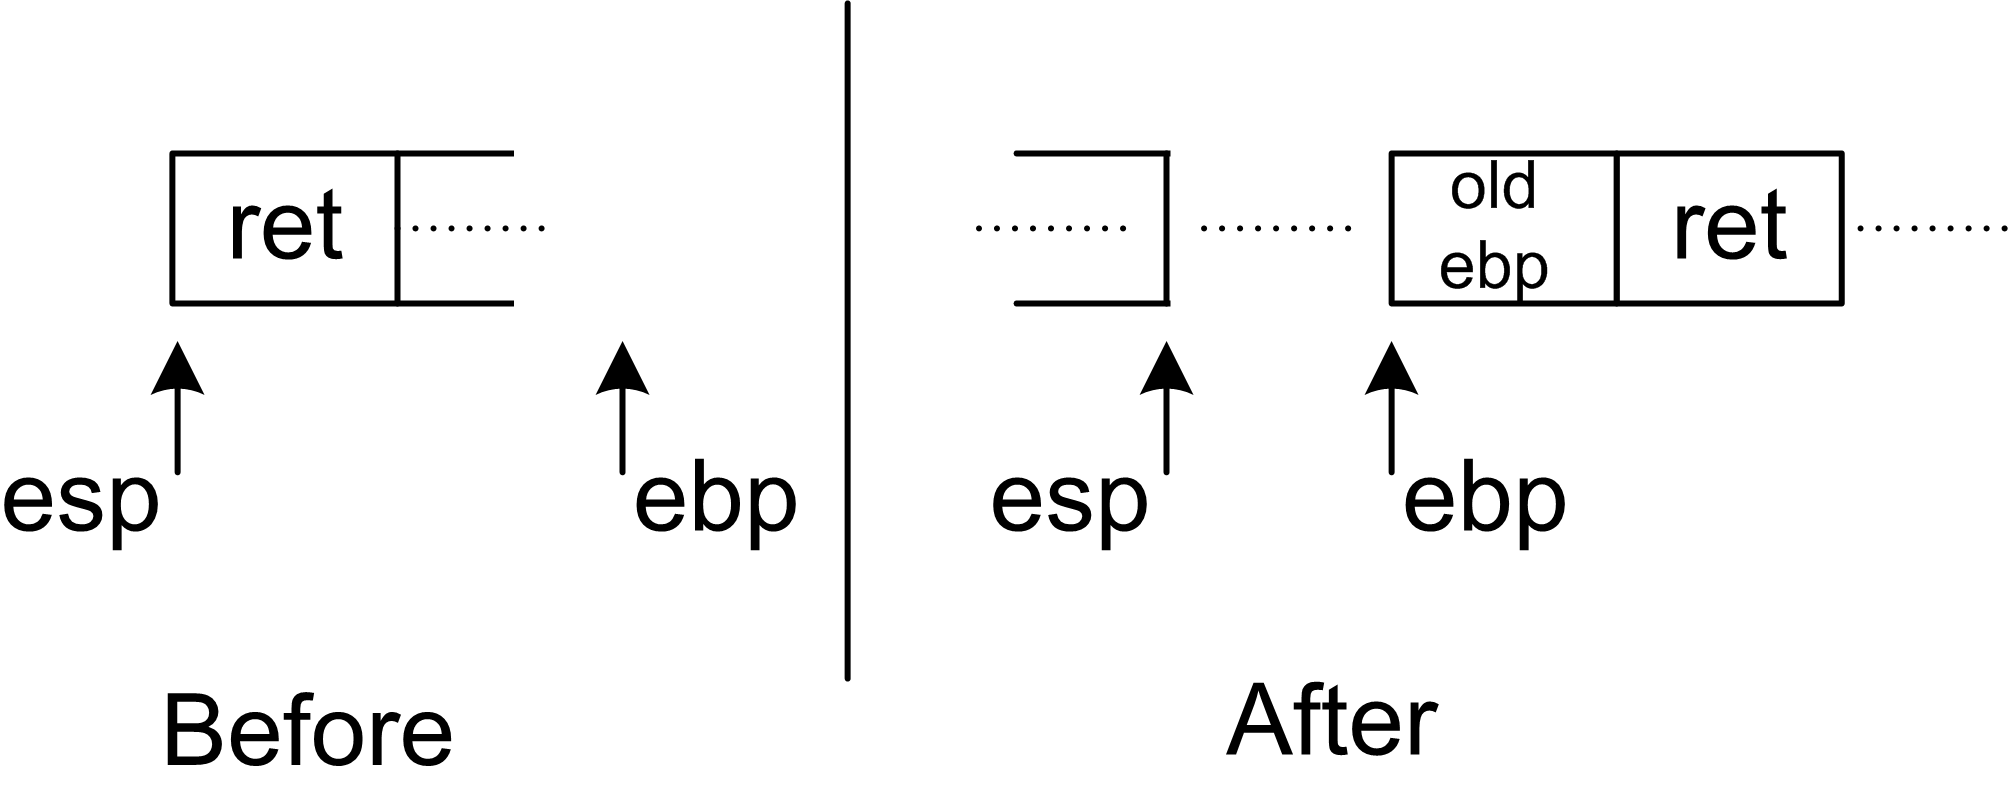
\includegraphics{fig_entry}
\caption{The state of the stack before and after 
|foldr| is entered.}
\label{fig_entry}
\end{figure}

On exit, the function must:

\begin{enumerate}
\item Place its result in a well-known location.
\item Restore the stack registers.
\end{enumerate}

\noindent
Every function returns its result in #eax#, which takes care of step
1. Restoring the stack is a simple matter of setting #esp# to
#ebp#. The previous base pointer will now be on the top of the
stack. Popping this value to #ebp# restores the stack to its previous
state. The return address for the function is now on top of the stack,
and a #ret# instruction is executed.

The code implementing this for the |Nil| arm in |foldr| is:

\begin{verbatim}
    movl -12(%ebp), %eax
    movl %ebp, %esp
    popl %ebp
    ret
\end{verbatim}

\noindent
and the state of the stack, before and after, is shown in figure \ref{fig_exit}.

\begin{figure}\centering
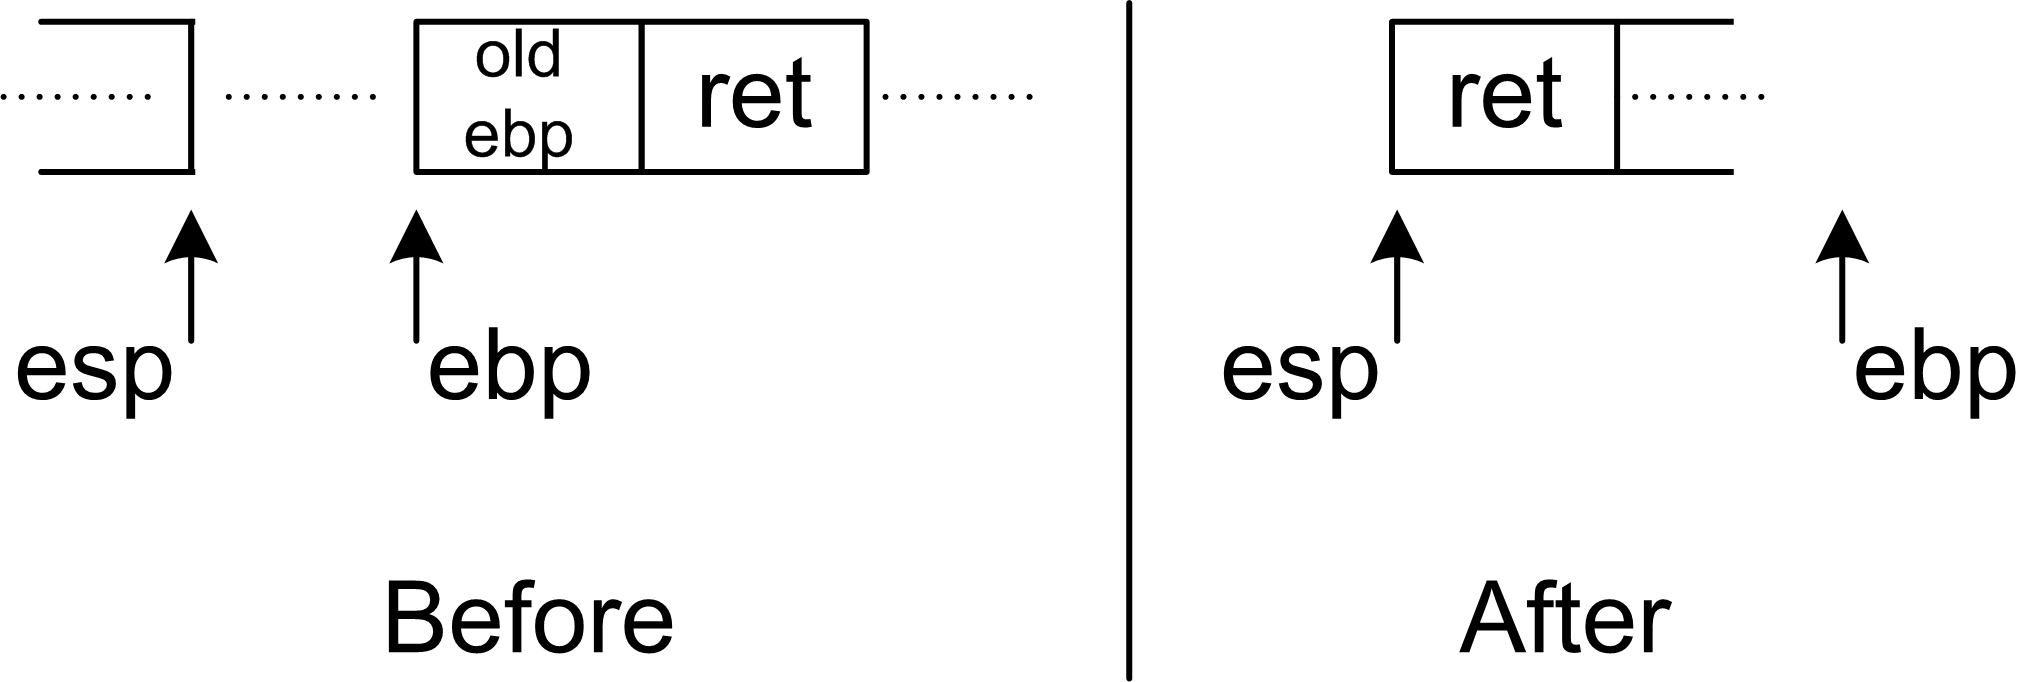
\includegraphics{fig_exit}
\caption{The state of the stack before and after 
|foldr| is exited.}
\label{fig_exit}
\end{figure}

\subsubsection{Reserved Registers}

There are only two registers which are reserved at all times. The
current closure will always be found in #edi#, while the current
argument will be in #esi#. #edx# and #ecx# are generally used as
temporary storage. #ebp# and #esp# retain their standard
meaning. Finally, #eax# is used to return results from functions.

\subsubsection{Allocation}

The runtime exports a C function, #alloc#, which allocates values on
the heap for Caffeine programs. #alloc# takes only one argument, a
pointer to the info table. The word prior to the address given is used
to determine how many words to allocate. After the object is
allocated, the value found at the address given is written into the
first word of the allocated value. If a closure is being allocated,
then the value written in will be the address of the destination
function for the closure. If it is a data constructor, then the tag
for that constructor will have been written. In either case, #alloc#
returns the address of the allocated object to the calling function.

\subsubsection{Case Analysis}
|FailT| implements case analysis in the IL. At the assembly level,
case analysis is implemented by comparing tag values. As described
above, the head of the heap object representing a data value holds the
tag for the constructor of that value. Case analysis is then a simple
comparison. For example, the check for |Z| constructor in |add Z b =
b| is simply:

\begin{verbatim}
    cmpl $0x27f, %ecx
    jnz lab76
\end{verbatim}

In this case, #ecx# holds the value to test and #lab76# is the label
to jump to if the test fails. The literal value #$0x27f# represents
the %$
 |Z| constructor.

\section{Remaining Work}

Much remains to be done to make Caffeine a viable compiler for the
Habit language. Besides support for features such as classes and
instances, code generation also needs considerable work. The compiler
was designed with reuse in mind, however. The output of each
compilation stage is not hidden behind an executable. The
|Habit.Compiler.Register.Compiler| module exports |compile|, which gives the
list of |Group| values described in section
\ref{subsec_input_output}. |Habit.Compiler.X86.Compiler| also exports
a |compile| function, which returns a list of assembly
instructions. Some possible improvements include inserting an
optimization pass after the first stage or replacing the assembly
generator altogether.

\end{document}
